\documentclass[12pt]{article}
\usepackage[spanish]{babel}
\usepackage[utf8x]{inputenc}
\usepackage{fancyhdr}
\usepackage[shortlabels]{enumitem}
\usepackage{setspace}
\usepackage[hidelinks]{hyperref}
\usepackage{graphicx}
\usepackage{natbib}
\usepackage{listings}
\usepackage{float, tikz,geometry,graphicx}
\usepackage{tabularx, enumitem}
\usepackage{listings}
\usepackage[T1]{fontenc}
\usepackage{beramono}
\usepackage{natbib}
\usepackage{longtable}
\usepackage{multirow}

\setcounter{tocdepth}{2} % Show sections

\definecolor{codegreen}{rgb}{0,0.6,0}
\definecolor{codegray}{rgb}{0.5,0.5,0.5}
\definecolor{codepurple}{rgb}{0.58,0,0.82}
\definecolor{backcolour}{rgb}{0.95,0.95,0.92}

\lstdefinestyle{mystyle}{
    backgroundcolor=\color{backcolour},   
    commentstyle=\color{codepurple},
    keywordstyle=\color{orange},
    numberstyle=\tiny\color{codegray},
    stringstyle=\color{codegreen},
    basicstyle=\ttfamily\footnotesize,
    breakatwhitespace=false,         
    breaklines=true,                 
    captionpos=b,                    
    keepspaces=true,                 
    numbers=left,                    
    numbersep=5pt,                  
    showspaces=false,                
    showstringspaces=false,
    showtabs=false,                  
    tabsize=2
}

\author{Anthony Aguilar \and Christian Ledgard \and Alexander Baldeon}
\title{Proyecto - Teoría de la Computación}

% encabezados
\lhead[]{CS2101- UTEC \\Teoría de la Computación}
\chead[]{2020-1}
\rhead[]{Prof. Juan Gutierrez Alva \\jgutierreza@utec.edu.pe}
\renewcommand{\headrulewidth}{0.5pt}

% pie de pagina
\rfoot[]{}
\renewcommand{\footrulewidth}{0pt}
\renewcommand{\labelenumii}{\theenumii}
\renewcommand{\theenumii}{\theenumi.\arabic{enumii}.}

\pagestyle{fancy}



\begin{document}
  \begin{titlepage}
    \centering
    {\bfseries\LARGE Universidad de Ingeniería y Tecnología\par}
    \vspace{2cm}
    {\scshape\Large Ciencia de la Computación\par}
    \vspace{3cm}
    {\scshape\Huge Natural Language Processing with Context Free Grammar\par}
    \vspace{3cm}
    {\itshape\Large Proyecto - Teoría de la Computación\par}
    \vfill
    {\Large Autores: \par}
    {\Large Christian Ledgard Ferrero\par}
    {\Large Anthony Aguilar Sanchez\par}
    
    \vfill
    {\Large Junio 2020 \par}
  \end{titlepage}
  \thispagestyle{fancy}

\tableofcontents

\newpage

\section{Introducción}
 Hoy en día la tecnología está presente en muchos ámbitos de nuestra sociedad. Desde vehículos que se manejan por sí solos hasta en nuestros celulares que nos permiten estar más comunicados que nunca. Unos de los avances más significativos en los últimos tiempos son los asistentes virtuales como Siri, Alexa, Google Assistant, entre otros. ¿Alguna vez se han preguntado cómo estos sistemas organizan y analizan nuestras oraciones para ponerlas en un determinado contexto? Una posible implementación es utilizar \textbf{gramáticas independientes del contexto} para organizar y luego generar un árbol de \textit{"parseo"} con la oración. Esto se logra al tener un léxico y una gramática previamente definida.

\section{Alcance}
En nuestro proyecto nosotros realizaremos una investigación aplicada en donde desarrollaremos un algoritmo simple para realizar un parser  de acuerdo a un léxico y gramática previamente definida. Utilizaremos diversas fuentes \cite{box_2018}, \cite{L5CFG_2017}, \cite{NLPOverview}, \cite{CFGandParsing_2015}, \cite{CFGWiki}, \cite{CYKAlgorithmWiki}, \cite{EPWiki}, \cite{LRParser} y \cite{LLParser}. 

\section{Definición del Problema}
Cómo dividir una oración, utilizando gramáticas independientes del contexto, para que el computador pueda interpretarlas correctamente. ¿Casos de ambigüedad? ¿Qué hacer en determinados casos?


\section{Estado del Arte}
El inicio del procesamiento de lenguaje natural suele remontarse a 1950 cuando Alan Turing publicó el articulo 'Computing Machinery and Intelligence' donde propone lo que conocemos como el test de Turing, un criterio de inteligencia.
\\
Una de las primeras aplicaciónes del NLP ocurrió en 1954 e involucro la traducción de 60 oraciones rusas al inglés.
\\
En los 1960´s ELIZA y SHRDLU fueron sistemas capaces de comunicarce con  humanos.
\\
Existen al menos 4 algoritmos de parsing:
\begin{enumerate}
    \item El algoritmo CYK (Cocke–Younger–Kasami)
    \begin{enumerate}
        \item Solo trabaja con CFG en la forma normal de chumsky
        \item El peor de los casos es $O(n^3 . |G|)$ time. Donde $n$ es el tamaño de la cadena y $|G|$ es el tamaño de la gramática $G$ lo que lo hace uno de los mas eficientes en el peor de los casos.
    \end{enumerate}
    \item Earley parser
    \begin{enumerate}
        \item Trabaja con todas las gramáticas libres del contexto.
        \item Tiene un tiempo de ejecución $O(n^3)$ en el caso promedio,$O(n^2)$ en gramáticas no ambiguas y $O(n)$ para CFG deterministas.
    \end{enumerate}
    \item LR parser (Left-to-right, Rightmost derivation in reverse)\\
    Son tipos de bottom-up parsers que analizan DCFG en tiempo lineal.
    \begin{enumerate}
        \item LALR parser
        \item Canonical LR parser
        \item Minimal LR parser 
        \item GLR parser
    \end{enumerate}
    
    \item LL parser (Left-to-right, Leftmost derivation)\\
    Es un top-down parser para un subset de CFG
\end{enumerate}

\section{Propuestas}
\begin{itemize}
    \item Implementar y analizar un algoritmos de parseo para construir una gramática independiente del contexto bajo una gramática y un lenguaje dado.
    \item Analizar posibles implementaciones y soluciones en casos de ambigüedad y presentar propuestas utilizadas actualmente por grandes empresas como Amazon o Google.
\end{itemize}
\newpage

\section{Implementación de Algoritmos}



Para implementar los algoritmos CYK y Earley definimos primero que es una gramática.

\subsection{Clase Gramática}
Para la implementación de la estructura regla, la dividimos en 2 partes: Derecha e Izquierda. Ejemplo: izq -> der. La parte izquierda estará definida por un string y la derecha por un vector de strings. Asimismo, creamos la clase gramática que almacenará en un vector de punteros a reglas, todas las reglas a analizar.

\lstinputlisting[style=mystyle, language=C++]{codigo/gramatica.h}
%\lstinputlisting[style=c-style]{codigo/gramatica.cpp}
\newpage


\subsection{Algoritmo CYK}
El siguiente algoritmo, considerado 'bottom-up parsing', fue inventado por John Cocke, Daniel Younger y Tadao Kasami. Este solo opera con gramáticas en la forma normal de Chomsky \cite{CYKAlgorithmWiki}. 

Utilizando la notación Big O, el peor caso del algoritmo CYK es  
 ${\displaystyle {\mathcal {O}}\left(n^{3}\cdot \left|G\right|\right)}$ donde ${\displaystyle n}$ es la longitud de la cadena y ${\displaystyle \left|G\right|}$ es el tamaño de la gramática \cite{HopcroftUllman}. Esta complejidad hace que sea uno de los algoritmos más eficientes de parseo en términos del peor caso.

Cumpliendo con los estándares, utilizaremos programación dinámica para resolver el Algoritmo CYK. Conforme al pseudocódigo expuesto en la Figura \ref{fig:pCYK}, realizaremos la implementación en C++, orientada a objetos.

\begin{figure}[h!]
    \centering
    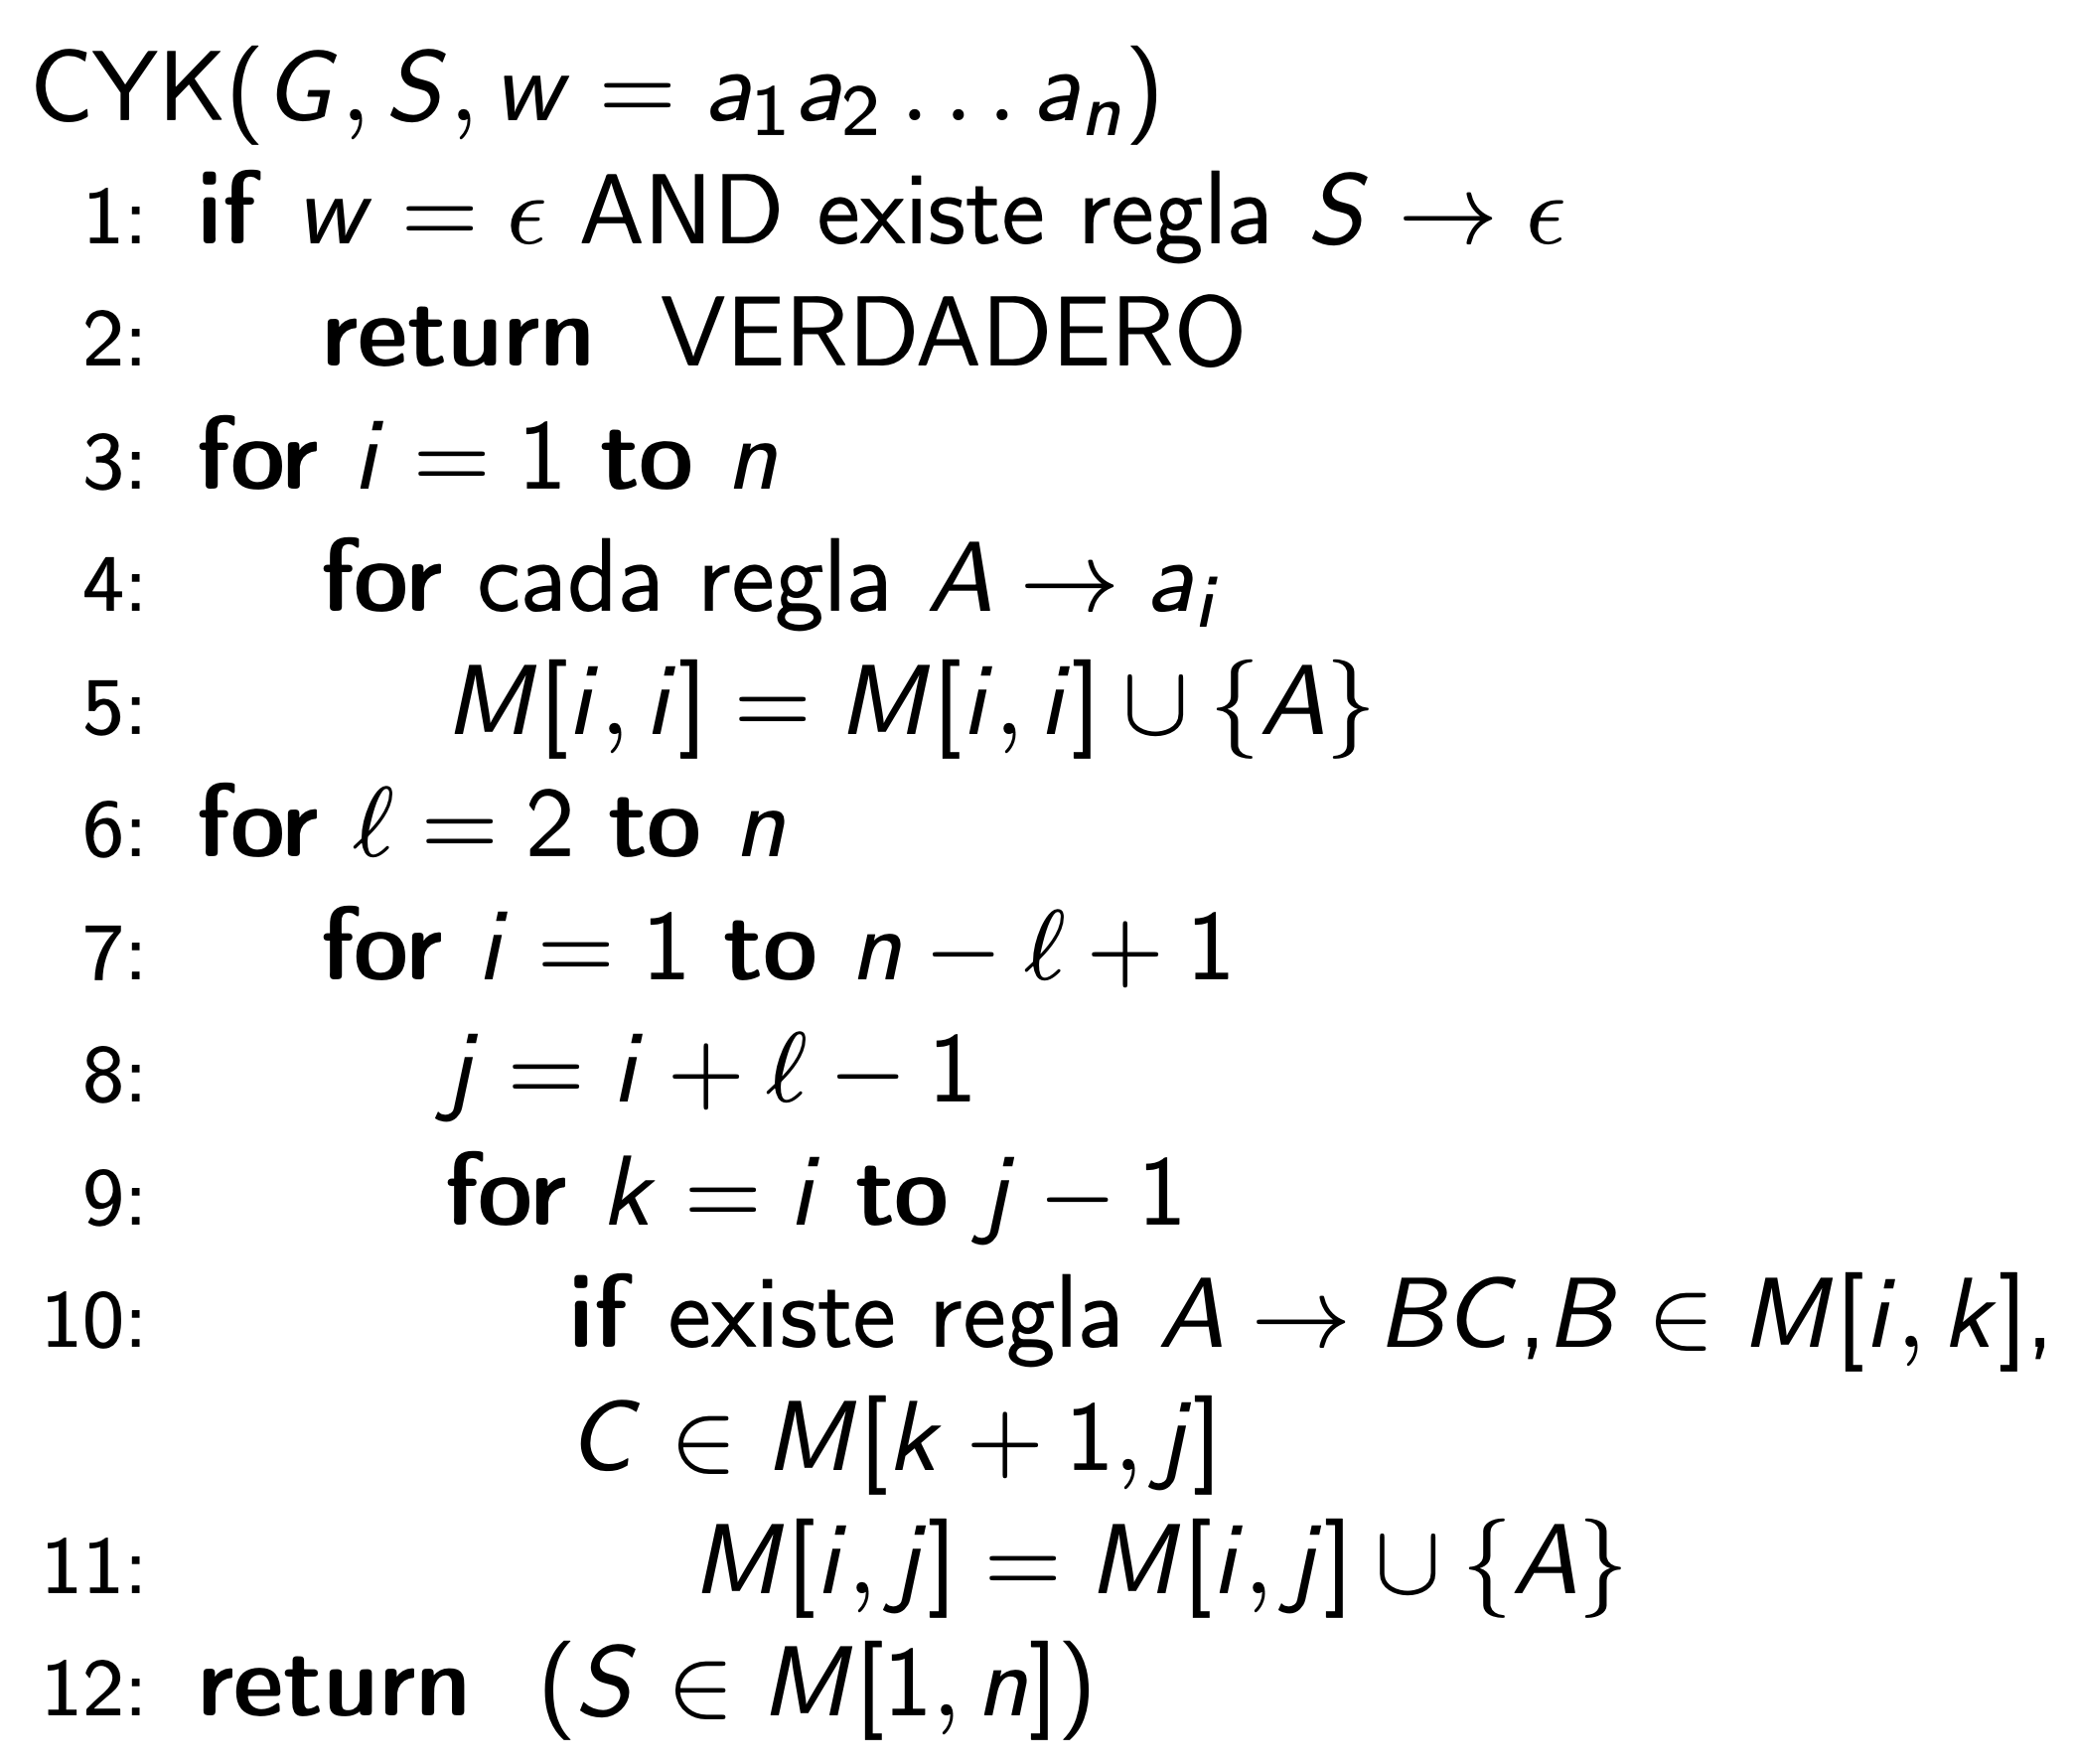
\includegraphics[width=250px]{img/pCYK.png}
    \caption{Pseudocódigo del algoritmo CYK}
    \label{fig:pCYK}
\end{figure} 

Nosotros creamos un array llamado matriz para almacenar el resultado ya procesado. Asimismo, en el método 'solve', ejecutaremos el algoritmo. Dicho método retornará un doble puntero, al puntero del array donde estará guardado nuestro resultado dinámico con la solución. También, en el método 'cadenaAceptada()', retornamos TRUE si la cadena es aceptada por el algoritmo, de lo contrario, retornaremos FALSE.

\lstinputlisting[style=mystyle, language=C++]{codigo/CYK.h}
%\lstinputlisting[style=c-style]{codigo/CYK.cpp}

\newpage


\subsection{Algoritmo Earley Parser}
A diferencia del algoritmo CYK el algoritmo de Earley es del tipo 'top-down' ya que éste evalúa si la cadena pertenece a la gramática empezando por la regla inicial y derivándola hasta obtener la cadena en el caso que ésta exista en la gramática.
\\\\
Para los siguientes párrafos $\alpha$, $\beta$ y $\gamma$ representan cualquier cadena de variables y símbolos de la gramática. $X$ y $Y$ representan variables de la gramática.Y $a$ representa cualquier símbolo de la gramática.
\\\\
Para lograr esta derivación se introduce una notación llamada 'dot-notation' o notación-punto $X \rightarrow \alpha \cdot \beta$. Esta notación indica que parte de una regla de la gramática ya ha sido reconocida (la parte a la izquiera del punto) y qué variable o símbolo se espera a continuación (la parte a la derecha del punto).
\\\\
Dada una cadena de tamaño $n$ se construye un array de tamaño $n+1$ donde cada posición en el array a partir de la posición 1 corresponde a un símbolo en la cadena correspondiendo la posición 0 al $\epsilon$ que precede a la cadena. Cada lugar en el array le corresponde a un conjunto de estados donde cada estado es una tupla que se construye a partir de una 'dot-notation' y la posición en el array donde 
ésta se originó $(X \rightarrow \alpha \cdot \beta, i)$. Llamamos al conjunto de estados que se encuentran en la posición $k$ $E(k)$.
\\\\

Este algoritmo consiste en repetir tres operaciones basadas en estos estados: predecir, escanear y  completar.

\begin{itemize}
    \item Predecir: para todos los estados en $E(k)$ de la forma $(X \rightarrow \alpha \cdot Y \beta,i)$, agregamos $(Y \rightarrow \cdot \gamma , k)$ a $E(k)$ para todas las producciones de la forma $Y \rightarrow \gamma$ en la gramática.
    \item Escanear: si $a$ es el siguiente símbolo a leer entonces para todos los estados en $E(k)$ de la forma $(X \rightarrow \alpha \cdot a \beta,i)$, agregamos $(X \rightarrow \alpha a \cdot \beta,i)$ a $E(k+1)$.
    \item Completar:  para todos los estados en $E(k)$ de la forma $(Y \rightarrow \gamma \cdot, i)$, buscamos todos los estados en $E(i)$ de la forma $(X \rightarrow \alpha \cdot Y \beta,j)$ y agregamos $(X \rightarrow \alpha Y \cdot \beta,j)$ a $E(k)$.
\end{itemize}

Notese que el tamaño de $E(k)$ puede aumentar de tamaño después de cada operación así que se tiene que realizar las respectivas operaciones a los nuevos estados generados por operaciones previas.

\lstinputlisting[style=mystyle, language=C++]{codigo/Earley.h}
%\lstinputlisting[style=c-style]{codigo/Earley.cpp}



\section{Hoy en la Industria: Análisis Experimental}
 Muchas de las grandes empresas que conocemos el día de hoy, como Google, Apple, Microsoft, entre otras, desarrollan su propia tecnología para interpretar un texto simple y analizarlo con el objetivo que el computador pueda interpretar el contexto de la oración. Por un lado podemos observar a empresas como Apple INC. que desarrollan un framework llamado 'NSLinguisticTagger' \cite{NSLinguisticTagger}, el gigante de Google desarolla 'Syntaxnet' \cite{SyntaxnetGH}, y muchas empresas suman y aportan más tecnologías. En este caso, analizaremos SyntaxNet puesto que en el 2016 la declararon Open Source. Esto significa que nosotros, los usuarios, podemos utilizar, cambiar y redistribuir el software, a cualquiera, para cualquier propósito, ya sea en su forma modificada o en su forma original \cite{OpenSource}.

Un gran problema al desarrollar este tipo de tecnologías es que el lenguaje que utilizamos nosotros, los seres humanos, tiene grandes niveles de ambigüedad (propiedad muy conocida al analizar las Gramáticas Independientes del Contexto). Google AI \cite{GoogleAISyntaxNet} nos menciona que es muy común encontrarse con oraciones de 20 a 30 palabras que cuenten con miles o cientos de miles posibilidades sintácticas. ¿Esto qué quiere decir? Que el computador tiene que buscar entre esas alternativas y encontrar la estructura más plausible dado el contexto. 

En este caso vamos a mencionar un ejemplo expuesto por Google AI \cite{GoogleAISyntaxNet}. 

\begin{figure}[h!]
    \centering
    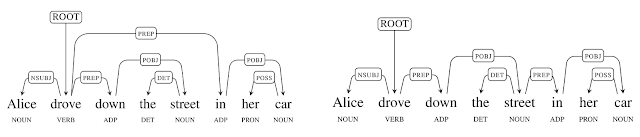
\includegraphics[width=\textwidth]{img/EjemploAmbiguedad.png}
    \caption{Ejemplo de Ambiguedad de Google AI \cite{GoogleAISyntaxNet}}
    \label{fig:AmbEjm}
\end{figure} 

En la siguiente oración: 'Alice drove down the street in her car.' (Alice condujo por la calle en su auto.) podemos obtener 2 interpretaciones: La correcta, señala que Alice está efectivamente manejando su auto, y la segunda nos indica que la calle está ubicada en el carro (posible sintácticamente, pero absurdo). Este es un claro ejemplo de ambigüedad donde el computador tiene que interpretar de manera correcta el contexto de la oración.

Google AI \cite{GoogleAISyntaxNet} también nos menciona que nosotros, como seres humanos, somos expertos en resolver estos problemas de ambigüedad. Somos tan expertos que ni siquiera notamos que estamos procesando esto en nuestro cerebro. El verdadero desafío está en que el computador realice las interpretaciones de manera correcta.

Nosotros sabemos que el problema de la ambigüedad no tiene una solución exacta. Por ello, todos los métodos para resolver la ambigüedad serán métodos de aprendizaje estadísticos, en el sentido de que intentan hacer una generalización inductiva a partir de los datos observados y utilizarlos para hacer inferencias con respecto a datos nunca vistos anteriormente \cite{Amb}. Estos métodos estadísticos, hoy en día, están considerados dentro de la rama de la Inteligencia Artificial. Roth \cite{Amb} nos menciona que existen cuatro aproximaciones para resolver el problema de la desambigüedad: The naive Bayes estimation (Duda ~ Hart 1973), Katz's back-off model, transformation based learning (Brill 1995) y el Decision Lists (Yarowsky 1995).

Todas estas aproximaciones buscan una superficie de decisión que sea una función lineal en el espacio de características. Esto quiere decir que los métodos asumen que el espacio está dividido en una función lineal, con la propiedad de que en una de  las regiones definidas, la predicción más probable es 0 y en la otra, la predicción más probable es 1. \cite{Amb}

Empresas como Google no son ajenas a estas técnicas de AI expuestas. Ellos utilizan estos métodos para resolver los problemas de ambigüedad. En este caso, 'SyntaxNet' utiliza redes neuronales para resolver el problema de la ambigüedad. Pero, ¿cómo lo hacen?. Google AI \cite{GoogleAISyntaxNet} nos señala que procesan una oración de izquierda a derecha en donde cada palabra de la oración es considerada en el algoritmo. Cabe recalcar que llegan a un punto donde encuentran varias soluciones posibles, pero debido a la ambigüedad, no pueden llegar a una decisión prematura. Por esta razón, utilizan un 'Beam search' (optimización del best-first search) para recorrer el grafo generado e ir descartando posibles hipótesis cuando existan varias otras hipótesis 'rankeadas' con un puntaje más alto y estas estén bajo consideración.

¿Que tan preciso es este modelo? Según Google AI \cite{GoogleAISyntaxNet} se ha logrado una precisión al 94\% después de probar el algoritmo con miles de oraciones en el idioma inglés. Asimismo, en un estudio con lingüistas se comprobó que los seres humanos tienen un 96\%-97\% de precisión. Lograr esta precisión es algo extraordinario, todavía no llegamos a la precisión humana pero estamos muy cerca. Con estos resultados esta tecnología puede aplicarse sin problema en diversas áreas.

Este nuevo modelo se encuentra en el siguiente 'paper' \cite{GoogleAISyntaxPaper} publicado por Google el 19 de marzo del 2016.
 \subsection{Decision List}
 Listas de decisión es un algoritmo usado para resolver el problema de ambigüedad en el análisis del lenguaje natural con un porcentaje de acierto de incluso más del 90\% en las ambigüedades más complicadas. El algoritmo consiste en 7 pasos:\cite{DecisionLists}
\begin{enumerate}
    \item Identificar las ambigüedades que se quieren resolver:\\
    Por ejemplo los significados de palabras francesas que llevan acento. \cite{DecisionLists}\\ 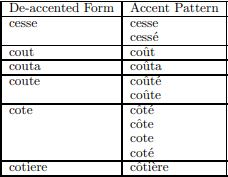
\includegraphics[]{img/listas/Listas_decision1.JPG}
    
    \item Recolectar los contextos para entrenar al algoritmo:\\
    Para esto es necesario construir oraciones que contengan las ambigüedades del punto anterior y que muestren diferentes contextos de uso. \cite{DecisionLists}\\
    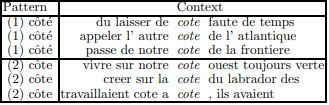
\includegraphics[]{img/listas/Listas_decision2.JPG}
    
    \item Medir como se distribuyen las palabras ambiguas:\\
    Para lograr esto se deben seguir las siguientes reglas:
    \begin{itemize}
        \item Por la palabra adyacente a la derecha de la ambigua será puntuada con $+1W$.
        \item Por la palabra adyacente a la izquierda de la ambigua, será puntuada con $-1W$.
        \item Por cada palabra a $k$ posiciones a la derecha de la ambigua será puntuada con $+kW$.
        \item Por cada palabra a $k$ posiciones a la izquierda de la ambigua será puntuada con $-kW$.
    \end{itemize}
    Entonces obtenemos una lista parecida a esta.\cite{DecisionLists}\\
    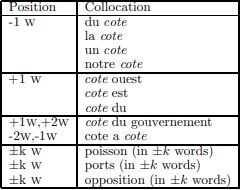
\includegraphics[]{img/listas/Listas_Decision3.JPG}
    
    \item Ordenar las tablas de forma descendente según la función de verosimilitud (log-likelihood\cite{log-likelihood}):\\
    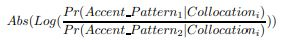
\includegraphics[]{img/listas/log-likelihood.JPG}\cite{DecisionLists}\\
    Dado que likelihood es una función de probabilidad necesitamos probabilidades que obtendremos de la data:\cite{DecisionLists}\\
    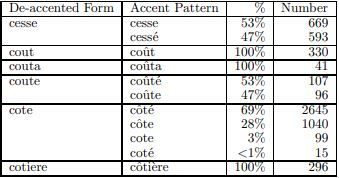
\includegraphics[]{img/listas/Listas_decision6.JPG}\\
    y terminaremos con una lista como esta:\cite{DecisionLists}\\
    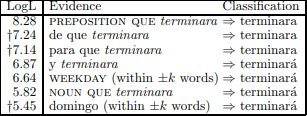
\includegraphics[]{img/listas/Listas_decision4.JPG}\\(notese que es de otro ejemplo)
    
    \item Opcionalmente podar e interpolar las listas
    \item Entrenar las listas para ambigüedades mas generales:\\
    Esto es cuando la palabra que causa la ambigüedad puede ser incluida en una clase o conjunto de palabras con usos similares.
    \item Usar las listas:\\
    Mientras se recorre el texto se revisa si a alguna palabra que se va leyendo le pertenece alguna lista de decisión, osea si se considera ambigua, ya sea de la misma palabra o de su clase, si es que pertenece a una clase. Si no se considera ambigua no pasa nada pero si sí, se recorre su lista hasta encontrar el mayor ranking que coincida con el contexto de la palabra ambigua.
\end{enumerate}

Análisis de la complejidad:
\begin{enumerate}
    \item Espacio:\\
    Supongamos que queremos analizar $n$ ambigüedades de las cuales el máximo de significados que alguna pueda tener es $k$ y queremos entrenar a la lista para reconocer estos significados en un máximo de $c$ contextos. Entonces tendríamos $n$ listas de tamaño $O(kc)$. Lo cual nos deja con una complejidad de $O(nkc)$ space.
    \item Tiempo:
    \begin{itemize}
        \item Para armar las listas:\\
        Obviando el paso opcional 5, para calcular la tabla solo se efectúan 2 operaciones: la medición de como se distribuyen las palabras ambiguas en el contexto y el ordenamiento de las listas según el resultado de la función log-likelihood.\\Para realizar la primera operación no se especifica ningún algoritmo así que supondremos que existe uno de complejidad $O(m)$ para puntuar las palabras de un contexto con un número máximo de $m$ palabras y sabiendo que la lista tiene un tamaño total de $n$ contextos podemos decir que la complejidad resultante de este paso es de $O(nm)$ time.\\Para la segunda operación sabemos que para una variable discreta, a diferencia de su forma para variables continuas, log-likelihood es una función matemática que no requiere del uso de métodos numéricos así que tiene una complejidad $\Theta(1)$ y para aplicarla a $n$ elementos de la lista se necesita $\Theta(n)$ time. Y una ves calculados estos valores deberá ser ordenada, para lo cual cualquier algoritmo de ordenamiento eficiente servira asi que supondremos uno de complejidad $O(nLog(n))$ time. Entonces $\Theta(n)+O(nLog(n))=O(nLog(n))$ time.
        \item Para usar las listas:\\
        Siguiendo las instrucciones indicadas en el paso 7 podemos intuir que se realiza un recorrido lineal a través de la lista lo cual nos daría un peor escenario de complejidad $O(n)$ time donde $n$ son las filas de la lista. Sin embargo, debido a que los elementos están ordenados de forma descendente en la probabilidad de ser el significado real obtenemos un escenario promedio de complejidad $O(1)$ time. Y con $p$ palabras ambiguas en la conseguimos la resolución de la ambigüedad en una cota inferior de $\Omega(p)$ y en una cota superior de $O(pn)$.
    \end{itemize}
\end{enumerate}

\section{Alternativas: Inteligencia Artificial}
 La inteligencia artificial es la mejor solución para resolver el problema de la ambigüedad. Al entrenar e implementar una red neuronal, podemos lograr precisiones casi similares a la de los seres humanos, como lo detallamos en la sección anterior.

\subsection{Implementación Simple de AI}

El objetivo de esta experimentación es poder transmitir un poco de lo que se puede hacer con esta tecnología. En este caso, implementaremos una pequeña red neuronal para identificar si una titular de una noticia contiene 'sarcasmo' o no. Para luego, finalizar el proyecto con algunos futuros cambios que se podrían hacer para adaptarlo a gramáticas.

La siguiente implementación fue creada por Rishabh Misra \cite{NLPinTensorFlow}.

\begin{lstlisting}[style= mystyle, language=Python]
import json
import tensorflow as tf

from tensorflow.keras.preprocessing.text import Tokenizer
from tensorflow.keras.preprocessing.sequence import pad_sequences
\end{lstlisting}

En este caso utilizaremos la librerías de TensorFlow para hacer esto posible.

\begin{lstlisting}[style= mystyle, language=Python]
vocab_size = 10000
embedding_dim = 16
max_length = 100
trunc_type='post'
padding_type='post'
oov_tok = "<OOV>"
training_size = 20000
\end{lstlisting}

En primer lugar, tenemos que definir ciertos parámetros como el tamaño del vocabulario, la longitud máxima de una oración y el tamaño de nuestro entrenamiento.

\begin{lstlisting}[style= mystyle, language=Python]
!wget --no-check-certificate \
    https://storage.googleapis.com/laurencemoroney-blog.appspot.com/sarcasm.json \
    -O /tmp/sarcasm.json
\end{lstlisting}

Para ese experimento, utilizaremos un archivo JSON con los títulares y si efectivamente ese titular es sarcástico o no. 

\begin{lstlisting}[style= mystyle, language=Python]
with open("/tmp/sarcasm.json", 'r') as f:
    datastore = json.load(f)

sentences = []
labels = []

for item in datastore:
    sentences.append(item['headline'])
    labels.append(item['is_sarcastic'])
\end{lstlisting}


Luego, interpretaremos el JSON y crearemos 2 listas con las oraciones y las etiquetas respectivamente.

\begin{lstlisting}[style= mystyle, language=Python]
training_sentences = sentences[0:training_size]
testing_sentences = sentences[training_size:]
training_labels = labels[0:training_size]
testing_labels = labels[training_size:]
\end{lstlisting}

Ahora, tenemos que dividir la data en 2 grupos. El grupo de entrenamiento y el grupo del testeo. Es muy importante asegurar que estos grupos contengan datos distintos. De lo contrario, obtendremos datos inexactos y violaremos principios de la red neuronal. 

\begin{lstlisting}[style= mystyle, language=Python]
tokenizer = Tokenizer(num_words=vocab_size, oov_token=oov_tok)
tokenizer.fit_on_texts(training_sentences)

word_index = tokenizer.word_index

training_sequences = tokenizer.texts_to_sequences(training_sentences)
training_padded = pad_sequences(training_sequences, maxlen=max_length, padding=padding_type, truncating=trunc_type)

testing_sequences = tokenizer.texts_to_sequences(testing_sentences)
testing_padded = pad_sequences(testing_sequences, maxlen=max_length, padding=padding_type, truncating=trunc_type)
\end{lstlisting}

El primer paso será convertir todas las palabras a un índice. Dicho índice estará compuesto por un diccionario que tendrá como LLAVE, la palabra y como VALOR, la frecuencia (cuantas veces se repite) en el texto.

Finalmente, nosotros sabemos que la red neuronal no procesa las palabras tal como son. Es por ello que utilizaremos el Tokenizer para convertir las palabras a números. Dichos números serán transformados a secuencias: listas 2D que almacenarán oraciones con la respectiva frecuencia de las palabras que componen la oración. 

\begin{lstlisting}[style= mystyle, language=Python]
model = tf.keras.Sequential([
    tf.keras.layers.Embedding(vocab_size, embedding_dim, input_length=max_length),
    tf.keras.layers.GlobalAveragePooling1D(),
    tf.keras.layers.Dense(24, activation='relu'),
    tf.keras.layers.Dense(1, activation='sigmoid')
])
model.compile(loss='binary_crossentropy',optimizer='adam',metrics=['accuracy'])
\end{lstlisting}

Ahora estamos llegando a la parte más importante del código: la definición del modelo. 'Embedding' consiste en la asociación de cada palabra con su sentimiento interpretado en un vector. Asimismo, $embedding\_dim$ define la dimensión del vector en cada palabra 

Finalmente, en la compilación es donde sucede la magia. Nosotros ya sabemos que para este ejemplo solo tenemos 2 posibilidades, de que el titular sea sarcástico o no, es por ello que utilizaremos $binary\_crossentropy$ en loss. Asimismo, utilizaremos el optimizador de Adam.

\begin{lstlisting}[style= mystyle, language=Python]
model.summary()
\end{lstlisting}
Ahora podremos observar el modelo en la figura \ref{fig:AI} .
\begin{figure}[h!]
    \centering
    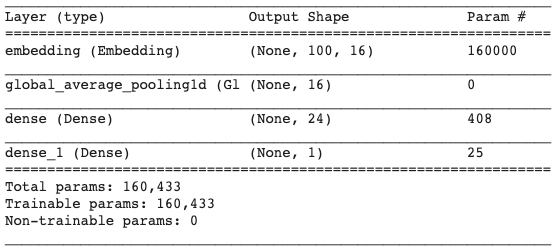
\includegraphics[width=250px]{img/AI/s.png}
    \caption{Summary del modelo AI}
    \label{fig:AI}
\end{figure} 

\begin{lstlisting}[style= mystyle, language=Python]
num_epochs = 30
history = model.fit(training_padded, training_labels, epochs=num_epochs, validation_data=(testing_padded, testing_labels), verbose=2)
\end{lstlisting}

Ahora realizaremos el entrenamiento de nuestra red neuronal. Para ello realizaremos 30 Epochs\footnote{Un Epoch es un término utilizado en Machine Learning que nos indica el número de pasadas del algoritmo al conjunto de entrenamiento.} a nuestro modelo AI. 


\begin{lstlisting}[style= mystyle, language=Python]
import matplotlib.pyplot as plt


def plot_graphs(history, string):
  plt.plot(history.history[string])
  plt.plot(history.history['val_'+string])
  plt.xlabel("Epochs")
  plt.ylabel(string)
  plt.legend([string, 'val_'+string])
  plt.show()
  
plot_graphs(history, "accuracy")
plot_graphs(history, "loss")
\end{lstlisting}

Ahora podremos visualizar el resultado de nuestro entrenamiento en la siguiente figura \ref{fig:AI} .
\begin{figure}[h!]
    \centering
    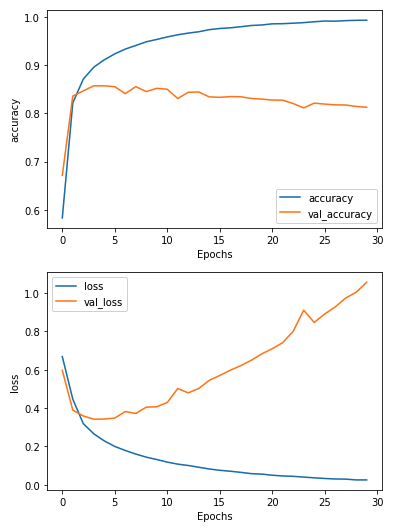
\includegraphics[width=250px]{img/AI/g.png}
    \caption{Resultado del entrenamiento de nuestra red neuronal}
    \label{fig:AI}
\end{figure} 

\begin{lstlisting}[style= mystyle, language=Python]
sentence = ["granny starting to fear spiders in the garden might be real", "game of thrones season finale showing this sunday night"]
sequences = tokenizer.texts_to_sequences(sentence)
padded = pad_sequences(sequences, maxlen=max_length, padding=padding_type, truncating=trunc_type)
print(model.predict(padded))
\end{lstlisting}

Finalmente, se podrá probar a continuación. Al correr model.predict(padded) obtenemos el siguiente vector: 
\begin{lstlisting}
[[9.0396011e-01]
 [8.0303380e-07]
 [4.1685485e-06]]\end{lstlisting}
 
 Esto quiere decir que existe una gran probabilidad de que la primera oración contenga sarcasmo, y una poca probabilidad que la segunda y tercera lo contenga.
 
 
\subsection{Futuras implementaciones y cambios para utilizar AI en la detección de ambigüedad}

La implementación mostrada en la última sección nos muestra el gran potencial de esta tecnología para resolver casos. Para poder aplicarlo con gramáticas, en la detección de ambigüedades, es necesario utilizar un modelo más complejo. Esto se debe a que ya no utilizaríamos como 'lable' a un número binario (0 y 1), por el contrario, tendríamos que utilizar otra estrategia. El arte de construir un modelo, está en definir de manera precisa el 'Embedding', con el objetivo de que los vectores generados cuenten con la presión deseada. Este arte, aplicado en el lenguaje natural, normalmente es propio de las grandes empresas; sin embargo en nuestra experimentación, nos empapamos con la tecnología detrás y la forma en la que esto funciona.


\section{GitHub}
Nuestro proyecto se encuentra almacenado en el repositorio GitHub. Para acceder, podrá hacer 
    \textbf{
        \href{https://github.com/christianledgard/Natural-Language-Processing-with-Context-Free-Grammar/}{click aquí} 
    }
.

\newpage

\bibliography{bibliografia}  
\bibliographystyle{ieeetr}

\end{document}
